

Im Anschluss an die erfolgte Konzeptphase und die Auswahl geeigneter Wirkkonzepte für die Teilfunktionen des Versuchsstandes werden die einzelnen Komponenten durch das Gestaltungskonzept einem Gesamtsystem zugeordnet. Der Entwurf legt dabei vorerst die grundlegende Gestaltung und Geometrie fest. Weiterhin werden strukturelle Elemente entwickelt, die zur Erfüllung der einzelnen Funktionen beitragen. Hier sollen die Ergebnisse dieser iterativen Phase dargestellt werden. 
\par
\vspace{\linespace}
Hauptdesigntreiber der äußeren Schirmhülle der Messkammer und damit der grundlegenden Struktur sind vor allem die Abmessungen. Die Auslegung soll in Anlehnung an die im \Abschnitt\ref{cha:2_sub_Genormte_Messverfahren} vorgestellten, geltende Normen erfolgen. Des Weiteren fließen ebenfalls die Erkenntnisse aus dem \Abschnitt\ref{cha:2_sub_Feldverlauf_in_Umgebung_eines_Dipols}, in dem die verschiedenen Feldverlaufszonen in der Umgebung eines Dipols betrachtet wurden, in die Festlegung der Hauptmaße ein.
\par
\vspace{\linespace}
Problematisch für die Bestimmung des Antennenabstandes zu den Probekörpern für eine Messung im Fernfeld ist, dass der Beginn der Fraunhofer Region und damit des Fernfeldes in verschiedenen Veröffentlichungen teils sehr unterschiedlich abgeschätzt wird. Weiterhin sind gegebene Berechnungsvorschriften oft mit der Aussage verbunden, dass der Abstand deutlich größer als der berechnete Grenzwert sein sollte. Dabei wird nicht näher spezifiziert, um welchen Faktor der Abstand erhöht werden sollte. In der \Tabelle\ref{tab:3_Fernfeldabstaende} sind die unterschiedlichen Fernfeldgrenzen für eine Frequenz von \SI{1}{\giga\hertz} basierend auf den referenzierten Publikationen aufgeführt. Da die Wellenlänge mit steigender Frequenz abnimmt, wird nach \Abschnitt\ref{cha:2_sub_Feldverlauf_in_Umgebung_eines_Dipols} der Abstand des Fernfeldes zum Dipol ebenfalls kleiner. Damit stellt die Abschätzung mit \SI{1}{\giga\hertz} den oberen Wert für die notwendige Ausdehnung der Messkammer dar.
\par
\vspace{\linespace}


\begin{table}[ht]
    \centering
    %\renewcommand{\arraystretch}{1.3}
    \caption{Fernfeldabstände für $f=1\,\si{\giga\hertz}$ auf Grundlage unterschiedlicher Veröffentlichungen}\label{tab:3_Fernfeldabstaende}
    \vspace{\tablespace}
    \begin{threeparttable}
    \begin{tabular}{@{\hspace{0.5cm}} p{5.5cm} R{1.3cm} @{,} p{0.5cm} @{m} p{1cm} p{0.5cm} p{1.5cm}}
    \toprule
        \textbf{Berechnungsvorschrift} & \multicolumn{3}{c}{\textbf{Fernfeldabstand}} & \multicolumn{2}{c}{\textbf{Quelle}}  \\   %\footnotemark[1]
    \midrule
        $r \gg \lambda / 2 \pi$  &     $\gg0$&05  &&&  \cite{Klassische_Elektrodynamik} \\
        $r \geq D^2 / \lambda$  &     $\geq0$&14  &&& \cite{NASA_SP-3067}\footnotemark[1] \\
        $r > 5 \lambda / 2 \pi$ &     $>0$&24  &&&  \cite{EMV, EMV-gerechtes_Geraetedesign} \\
        $r \geq 2 D^2 / \lambda$&     $\geq0$&27  &&&  \cite{Antenna_Theory}\footnotemark[1] \\
        %$r > 4 \lambda$         &     1&2   &&&  \cite{Bundesnetzagentur_Glossar_Nahfeld} \\
        DIN EN 61000-4-3, VG 95373-15         &     1&0   &&& \cite{DIN_EN_61000-4-3}\footnotemark[2]~\cite{VG_95373_15} \\
        IEEE 299                &     1&7   &&& \cite{IEEE_299} \\
        DIN EN 61000-5-7        &     2&0   &&& \cite{DIN_EN_61000-5-7} \\
    \bottomrule
    \end{tabular}
    \begin{tablenotes}
    \footnotesize
    \item[1]Annahme: $D \approx 0,2\,\si{\meter}$ entsprechend der zu verwendenden Hornantennen
    \item[2]Mögliche Reduktion für $f\geq1\,\si{\giga\hertz}$
    \end{tablenotes}
    \end{threeparttable}
\end{table}


Für den Abstand der Proben zur Sendeantenne wurde auf Grundlage der Werte in \Tabelle\ref{tab:3_Fernfeldabstaende} ein Abstand von etwa \SI{1}{\meter} gewählt. Dies ist nach den meisten Abschätzungen schon deutlich im Fernfeldbereich und in Übereinstimmung mit den Normen~\cite{DIN_EN_61000-4-3, VG_95373_15}. Entsprechend der \Gleichungen\eqref{eq:2_elektrische_Feldvektoren} und~\eqref{eq:2_magnetische_Feldvektoren} sowie der \Abb\ref{fig:2_Feldwellenwiderstand} sind die Terme höherer Ordnung, die das reaktive und strahlende Nahfeld beschreiben, bei diesem Abstand und einer Frequenz von \SI{1}{\giga\hertz} vernachlässigbar und ihr Einfluss sinkt bei gleichem Abstand und steigender Frequenz noch weiter. 
\par
\vspace{\linespace}
Aus dem gewählten Antennenabstand ergibt sich eine gesamte Messkammerlänge von etwa \SI{2}{\meter} unter Beachtung der Antennenausdehung und der Höhe gängiger Absorberelemente~\cite{Telemeter_Produktseite, EMV-Support_Produktseite}, die mindestens hinter beiden Antennen zur Reduktion der Nebenkeulenreflektion angebracht werden sollten~\cite{Optimierung_Feldhomogenitaet, EM_Schirmung}. Bei einem Messausschnitt von $0,5 \times 0,5\,\si{\meter}$ in der Ebene der Prüflinge nach~\cite{DIN_EN_61000-4-3} ergibt sich eine Mindestbreite von circa \SI{1}{\meter} unter Beachtung der Absorber. Für die Höhe kann unter Berücksichtigung des Mindestabstandes der Prüflinge zum Boden von \SI{0,8}{\meter} nach~\cite{DIN_EN_61000-4-3, DIN_EN_61000-5-7} ein Wert von \SI{1,5}{\meter} inkl. Absorbern abgeschätzt werden. Um in beiden Richtungen orthogonal zur primären Ausbreitungsrichtung der Wellen ähnliche Feldeigenschaften an den Wänden der Messkabine und damit ähnliche Bedingungen für alle Absorber zu erzielen, wurden \SI{1,5}{\meter} als Breite und Höhe der Testkammer gewählt. 
\par
\vspace{\linespace}
Diese Maße bieten außerdem den Vorteil, dass keine Teilung der Modulwände in einer der Ausdehnungsrichtungen erfolgen muss, da die meisten angebotenen Sandwichpaneele bzw. Wabenkernplatten in entsprechender Breite und Länge zur Verfügung stehen. Dies reduziert die möglichen Stellen für Leckagen in der Schirmwand und den Fertigungsaufwand.
\par
\vspace{\linespace}
Die ersten Moden der Hohlraumresonanzfrequenzen liegen mit den abgeschätzten Abmessungen nach \Gleichung\eqref{eq:2_Hohlraumresonanzfrequenz} im Bereich zwischen \SI{125}{\mega\hertz} und \SI{160}{\mega\hertz} und damit deutlich unter der kleinsten Messfrequenz. Die Ausbildung stehender Wellen höherer Ordnung und sonstiger Reflektionen an den leitenden Schirmwänden muss dennoch durch Absorber unterdrückt werden.
\par
\vspace{\linespace}
Am häufigsten werden als Absorberelemente Kacheln aus gesintertem Ferrit in Form von kleinen Fliesen und Pyramidenabsorber aus PU-Schaum verwendet. Aufgrund der unterschiedlichen Wirkungsweise und Form sind diese jeweils für unterschiedliche Frequenzbereiche geeignet (vgl. \Abschnitt\ref{cha:2_sub_Daempfung_und_Absorption}). Ferrite werden bis zu Frequenzen von \SI{1}{\giga\hertz} eingesetzt, während Pyramidenabsorber im Allgemeinen nur bei höheren Frequenzen Anwendung finden. Eine Kombination beider ist ebenfalls möglich, erfordert nach \Abschnitt\ref{cha:2_sub_Daempfung_und_Absorption} aber eine genaue Abstimmung, um keine reflektive Grenzfläche zu schaffen. Aus wirtschaftlicher Sicht und weil die Leistungsfähigkeit einzelner Pyramidenabsorber auch im Bereich von \SI{1}{\giga\hertz} mit der von Kombinationen aus Ferrit und PU-Absorber vergleichbar ist, soll die Auskleidung mit einfachen Pyramidenelementen erfolgen. Die genaue Auswahl erfolgt im Rahmen der Ausarbeitung. Die Höhe von Absorbern mit ausreichender Reflektionsdämpfung beläuft sich auf etwa 10 -- \SI{20}{\centi\meter}~\cite{Holland_Shielding_Absorber, Telemeter_Produktseite, Eco_Messtechnik_Absorber}. Spezial- und Hochleistungsabsorber wurden für die vorliegende Anwendung aufgrund der hohen Kosten nicht in Betracht gezogen. 
\par
\vspace{\linespace} 
Die Positionierung der Proben ist ebenfalls ein wichtiger Teil des Entwurfes. Die Probekörper sind nicht groß genug, um den Koppelpfad zwischen den Antennen vollständig abzudecken. Dies macht einen Reflektor notwendigen, der den größten Teil der Wellen, die an den Proben vorbei in Richtung Empfangsantenne ausgesandt werden, reflektiert. So werden im Idealfall nur direkt durch die Proben verlaufende Wellenanteile von der Empfangsantenne aufgenommen. Die reflektierten Anteile verlieren ihre Energie an den Absorbern.   
\par
\vspace{\linespace}
Eine vollständige Trennung der Messkammer durch einen Reflektor ist aufgrund von entstehenden Resonanzen nach~\cite{Techniques_Shielding_Effectiveness_Far_Field_Simulation} nicht sinnvoll und reduziert die Vergleichbarkeit von Messungen mit solchen, die in anderen Messkabinen durchgeführt wurden. Entsprechend erfolgt eine Einfügung des Reflektorschirms in den direkten Koppelpfad der Antennen mit einer Mindestausdehnung von $0,5 \times 0.5\,\si{\meter}$~\cite{DIN_EN_61000-4-3}. Auf Grundlage der Betrachtungen im \Abschnitt\ref{cha:2_sub_Reflektion} kann als Reflektor eine Metallplatte mit möglichst hoher Leitfähigkeit genutzt werden.
\par
\vspace{\linespace} 
Das Wirkkonzept für den Einbau von Durchführungen wurde im \Abschnitt\ref{cha:3_sub_Durchfuehrungen} bewertet. Bei einer gewählten Höhe der Messkammer von etwa \SI{1,5}{\meter} ist eine aufrecht begehbare Tür ohnehin nicht möglich, sodass aus Gründen des günstigeren Aufbaus das lichte Maß so gewählt wurde, dass eine Interaktion mit den Antennen und das Einbringen neuer Proben gut möglich ist. Das Betreten des Teststandes sollte nur in Ausnahmefällen bzw. im Rahmen des Aufbaus möglich sein. Bezüglich der erreichbaren Schirmdämpfung spielen das lichte Maß oder das Türblattaußenmaß nur dahingehend eine praktische Rolle, als dass auf der gesamten Wirkfläche ein möglichst gleichmäßiger Anpressdruck an die HF-Dichtungen erreicht wird. Mit der Größe des Türblattes steigt die Anzahl notwendiger Haltepunkte bzw. das notwendige Flächenträgheitsmoment zum Gewährleisten einer ebenen Wirkfläche. Weiterhin müssen mit steigendem Gewicht des Türblattes natürlich auch alle Befestigungen massiver ausgeführt werden. Als Kompromiss zwischen diesen drei Optimierungszielen wurden $700 \times 700\,\si{\milli\meter}$ als lichtes Maß gewählt. Um Zugang sowohl zur Sende- als auch zur Empfangsantenne von außen zu gewährleisten, wurden in der Front der Messkammer zwei Türen vorgesehen.
% \par
% \vspace{\linespace}
% Die im Konzept der Durchführungen enthaltenen Kontaktfederstreifen bieten die beste erreichbare Schirmdämpfung im Vergleich zu anderen HF-Dichtungstypen~\cite{EM_Schirmung}. Gleichzeitig besitzen sie selbstreinigende Eigenschaften, denn aufgrund der Relativbewegung zwischen Rahmen und Dichtung werden Oxid- und andere Oberflächenschichten bei jedem Schließvorgang entfernt und es entsteht ein sauberer Kontakt mit geringem Kontaktwiderstand. Im Rahmen dieses Projektes sind die hohen Kosten im Vergleich zu anderen Dichtungen der hauptsächliche Nachteil, was jedoch durch ihre hohe Beständigkeit teilweise relativiert wird. Um einen guten Kontakt sicherzustellen, sind bei Verwendung von Beryllium-Kupfer-Kontaktferderstreifen höhere Anpresskräfte notwendig als bpsw. bei Elastomerdichtungen.  
\par
\vspace{\linespace}
Für die Durchführungen von Leitungen durch die Schirmwand und in die Messkammer gibt es mehrere Möglichkeiten. Die einfachste ist die Nutzung einer Eigenschaft von Hohlwellenleitern, der sogenannten Cut-off-Frequenz oder kritischen Frequenz $f_k$ mit der zugehörigen kritischen Wellenlänge $\lambda_k$ (vgl. \Abschnitt\ref{cha:2_subsub_Hohlwellenleiter}). Unterhalb dieser Frequenz ist in einem Hohlwellenleiter gegebener Geometrie \mbox{keine} Wellenausbreitung möglich und es findet eine aperiodische Dämpfung statt. Bei der Nutzung als \mbox{Kabeldurchführung} kann aus der höchsten Einsatzfrequenz eines Schirms die notwendige Geometrie abgeschätzt werden. Nach \Tabelle\ref{tab:2_Grenzwellenlaengen_Hohlleiter} ergibt sich für einen Kreisquerschnitt der größtmögliche Durchmesser für ein Kabel, welches in den Schirm geführt werden soll. Für \SI{18}{\giga\hertz} als höchste Einsatzfrequenz sind dies etwa

\begin{equation}
    d(18\,\si{\giga\hertz}) \approx \frac{\lambda(18\,\si{\giga\hertz)}}{1,305} = \frac{c_0}{18\,\si{\giga\hertz}\cdot 1,305} \approx 0,0127 \; \si{\meter}
\end{equation}

als größter Durchmesser für eine Kabeldurchführung mittels Hohlwellenleiter. Unter Beachtung, dass die kritische Frequenz im Anwendungsfall noch deutlich unter der höchsten Einsatzfrequenz liegen sollte~\cite{EM_Schirmung}, eignet sich diese Methode aufgrund des geringen möglichen Durchmessers nicht zur Durchführung der geschirmten Signalkabel vom \ac{VNA} zu den Antennen. Hinzu kommt, dass eine niederohmige Verbindung des Kabelschirmes mit der Schirmwand, wie sie bei der Durchführung geschirmter Kabel notwendig ist~\cite{EM_Schirmung, EMV}, in diesem Fall nur durch das Anlöten des Kabelschirmes zu erreichen wäre.
\par
\vspace{\linespace}
Am besten geeignet für die Einführung der HF-Kabel in das Gehäuse sind beidseitige Konnektoren mit einem Flansch zur Befestigung an der Schirmhülle. Hierdurch erfolgt eine lösbare Verbindung der Kabelschirme mit der äußeren Schirmwand ohne den Kabelschirm schädigen zu müssen. Dies bietet außerdem den Vorteil, dass die Antennenkabel unabhängig vom \ac{VNA} stets in der Messkammer verbleiben können und der \ac{VNA} mit wenigen Handgriffen anderweitig genutzt werden kann. 
\par
\vspace{\linespace}
Um bei den gewählten Abmessungen einen guten Zugang zu den Öffnungen zu gewährleisten, wird ein Untergestell aus Aluminiumprofilen genutzt, welches den Teststand auf eine gut erreichbare Höhe hebt und außerdem mithilfe von Rollen eine einfachere Positionierung erlaubt. An der Auflagefläche der Bodenplatte werden Verstrebungen so vorgesehen, dass auch bei Betreten des Versuchsstandes die Verformung der Grundplatte minimiert wird und elastisch bleibt.
\par
\vspace{\linespace}
In der \Abb\ref{fig:3_Entwurf_CAD} ist das Gestaltungskonzept mit einer Ansicht des CAD-Modells veranschaulicht. 
\par
\vspace{\linespace}\vspace{\linespace}


\begin{figure}[ht]
    \centering
    \hspace*{2cm}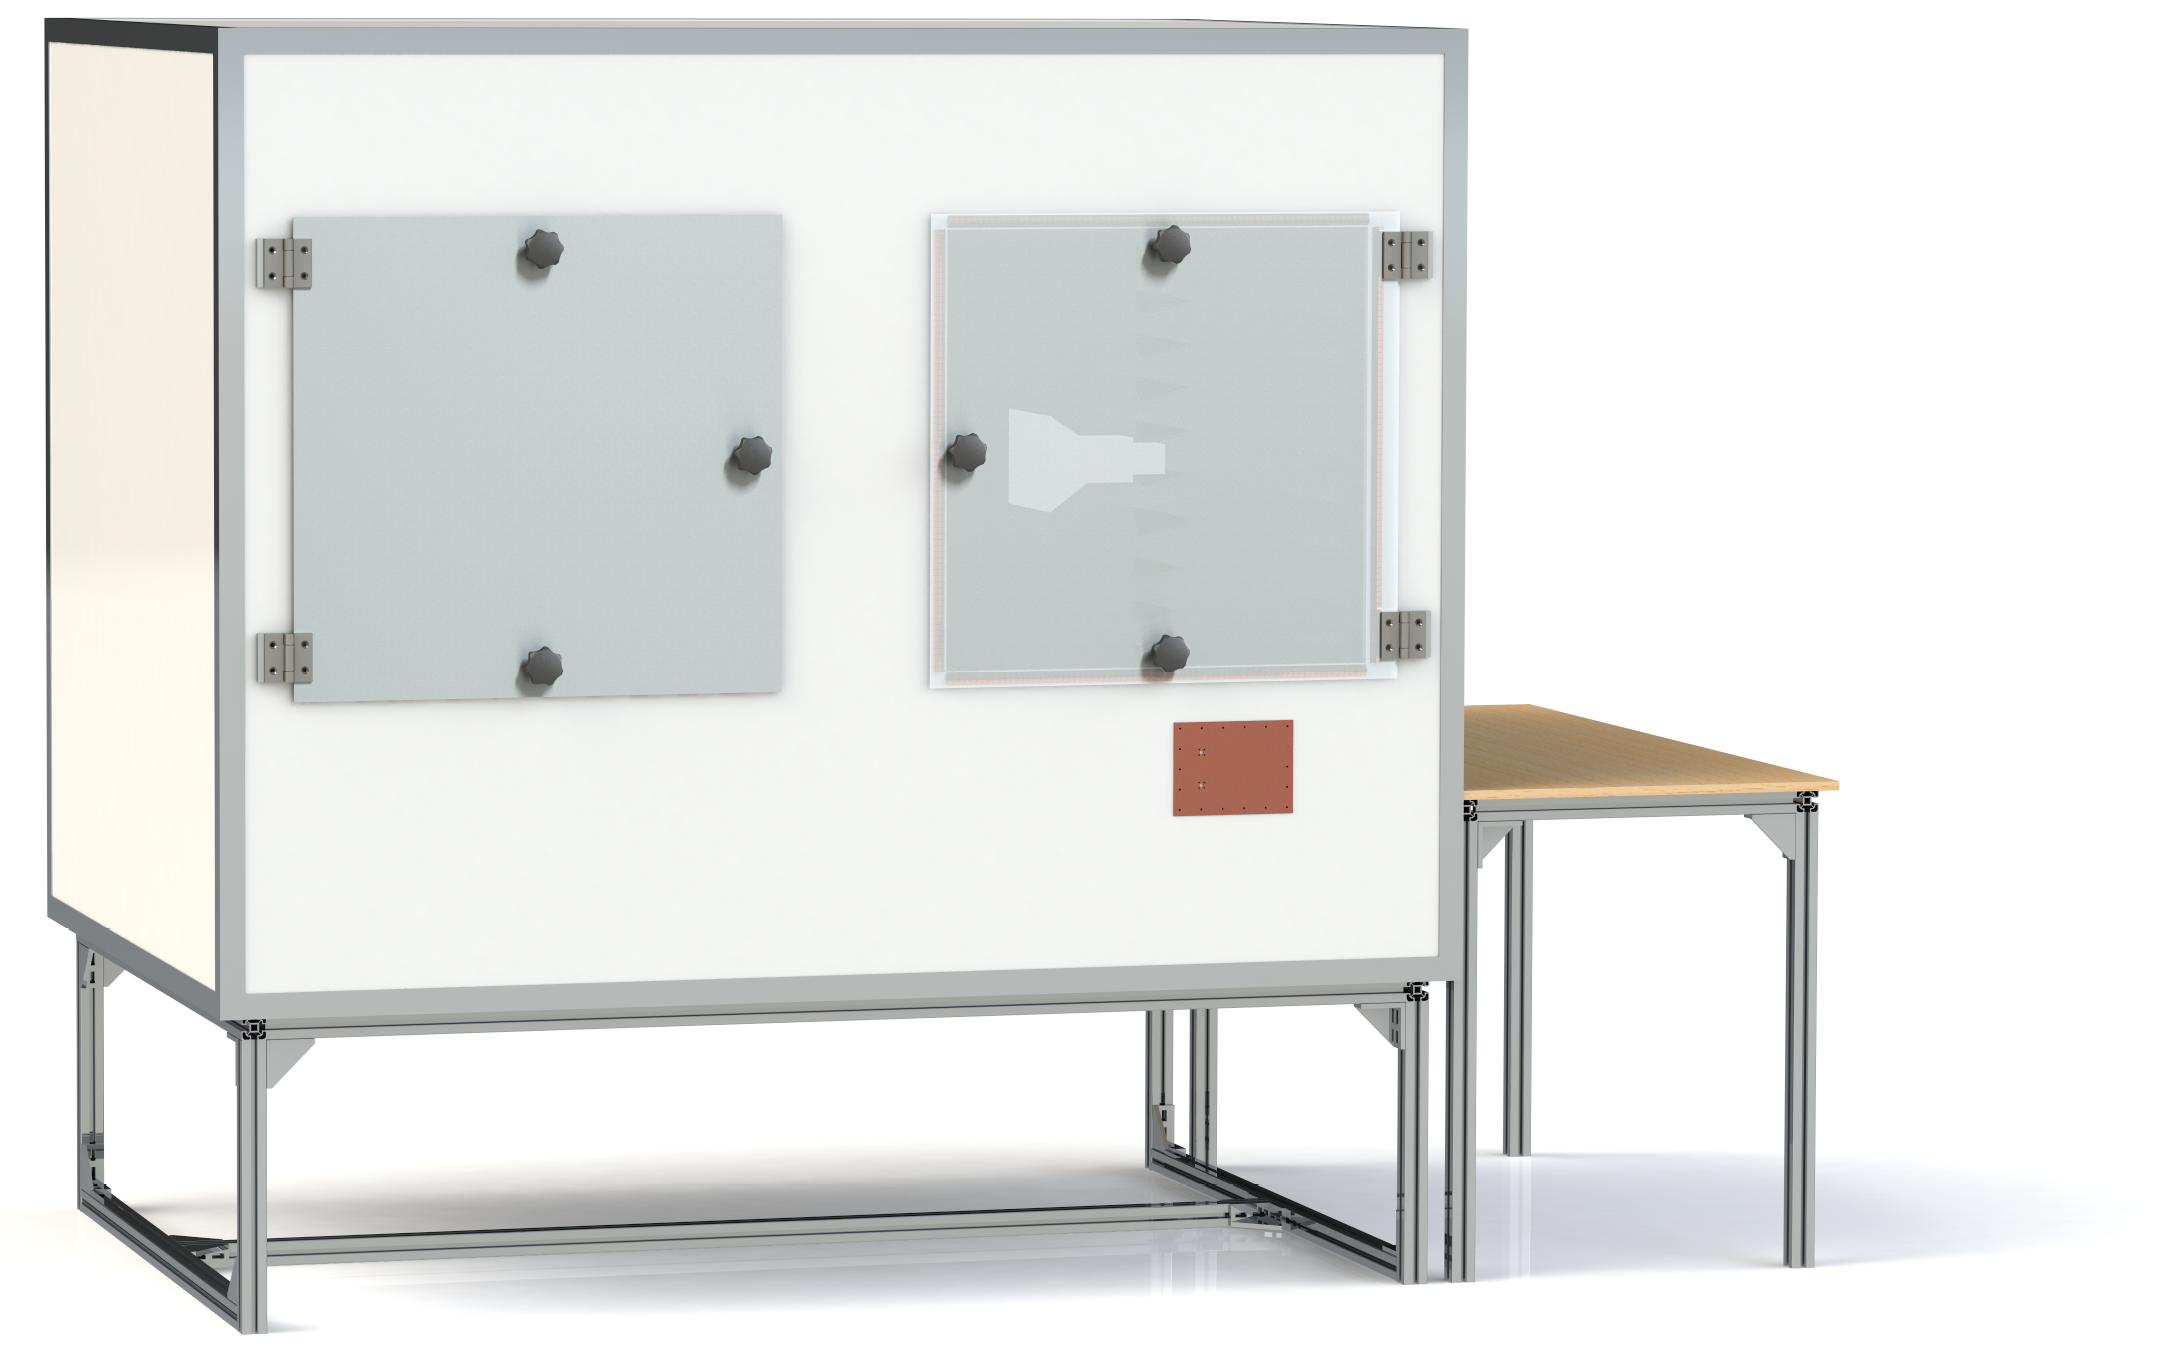
\includegraphics[width = .7\textwidth, trim = 0cm 0cm 1cm 0cm, clip]{Abbildungen/Kapitel3/Absorberkammer_Frontansicht.png}
    \caption{CAD-Modellansicht des Versuchsstandes}
    \label{fig:3_Entwurf_CAD}
\end{figure}



%Türen

%Dichtungen

%Kabeldurchführungen

%Gestell

%Beleuchtung









